


\begin{center}
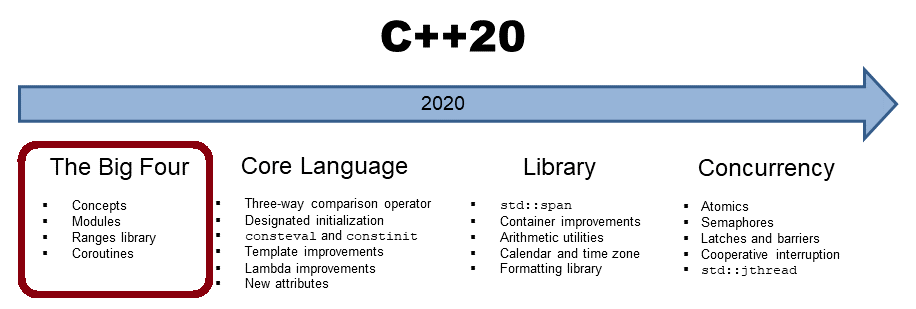
\includegraphics[width=1.0\textwidth]{content/2/chapter3/images/2.png}\\
每一个特性都会改变我们使用C++编程的方式。
\end{center}

\subsubsubsection{3.1.1\hspace{0.2cm}概念}

使用模板的泛型编程,使其能够定义可用于各种类型的函数和类。因此,使用错误类型实例化模板的情况并不少见,可能会看到长达数页的编译错误。这个问题可以通过概念解决,概念可编写编译器检查模板参数的需求,并彻底改变开发者思考和编写泛型代码的方式。原因如下:

\begin{itemize}
\item 
模板参数的需求成为其公共接口的一部分。

\item 
函数的重载或类模板的特化可以基于概念。

\item 
因为编译器根据给定的模板参数检查已定义的模板形参需求,所以我们得到了更明显的错误消息。
\end{itemize}

这还没完。

\begin{itemize}
\item 
开发者可以使用预定义的概念,也可以自定义概念。

\item 
auto和概念的用法统一,可以用概念来代替auto。

\item 
若函数声明使用了概念,则自动成为函数模板。这样,编写函数模板就像编写函数一样简单。
\end{itemize}

下面的代码片段演示了简单概念Integral的定义和使用:

\hspace*{\fill} \\ %插入空行
\noindent
\textbf{Integral概念的定义和使用}
\begin{lstlisting}[style=styleCXX]
template <typename T>
concept Integral = std::is_integral<T>::value;

Integral auto gcd(Integral auto a, Integral auto b) {
	if( b == 0 ) return a;
	else return gcd(b, a % b);
}
\end{lstlisting}

Integral概念从其类型参数T中要求std::is\_integral<T>::value为true。std::is\_integral<T>::value是来自\href{https://en.cppreference.com/w/cpp/header/type_traits}{类型特征库}的值,在编译时检查T是否为整数。若std::is\_integral<T>::value计算为true,则一切正常;否则,将会看到相应的编译时错误。

gcd算法基于\href{https://en.wikipedia.org/wiki/Euclid}{Euclidean}算法确定最大公约数,代码使用缩写函数模板语法来定义gcd。这里,gcd要求参数和返回类型支持Integral概念。换句话说,gcd是一种对其参数和返回值提出要求的函数模板。当删除语法糖时,可以看到真正的gcd。

下面是语义等效的gcd算法,使用了require子句。

\hspace*{\fill} \\ %插入空行
\noindent
\textbf{required子句中使用Integral概念}
\begin{lstlisting}[style=styleCXX]
template<typename T>
requires Integral<T>
T gcd(T a, T b) {
	if( b == 0 ) return a;
	else return gcd(b, a % b);
}
\end{lstlisting}

require子句声明了对gcd类型参数的要求。

\subsubsubsection{3.1.2\hspace{0.2cm}模块}

模块的承诺很多:

\begin{itemize}
\item 
更快的编译时间

\item 
减少宏定义

\item 
表达代码的逻辑结构

\item 
淘汰头文件

\item 
摆脱丑陋的宏替换
\end{itemize}

这是一个简单的数学模块:

\hspace*{\fill} \\ %插入空行
\noindent
\textbf{数学模块}
\begin{lstlisting}[style=styleCXX]
export module math;

export int add(int fir, int sec) {
  return fir + sec;
}
\end{lstlisting}

表达式会导出模块math(第1行)是模块声明。将export放在函数add之前(第3行)导出函数。现在,模块的使用者可以使用它。

\hspace*{\fill} \\ %插入空行
\noindent
\textbf{使用数学模块}
\begin{lstlisting}[style=styleCXX]
import math;

int main() {
	add(2000, 20);
}
\end{lstlisting}

表达式import math导入math模块,并使导出的名称在当前作用域中可见。

\subsubsubsection{3.1.3\hspace{0.2cm}范围库}

范围库支持的算法有如下特征

\begin{itemize}
\item 
can operate directly on containers; you don’t need iterators to specify a range

\item 
can be evaluated lazily

\item 
can be composed
\end{itemize}

To make it short: The ranges library supports functional patterns.

The following example demonstrates function composition using the pipe symbol.

\hspace*{\fill} \\ %插入空行
\noindent
Function composition with the pipe symbol
\begin{lstlisting}[style=styleCXX]
int main() {
	std::vector<int> ints{0, 1, 2, 3, 4, 5};
	auto even = [](int i){ return i % 2 == 0; };
	auto square = [](int i) { return i * i; };
	
	for (int i : ints | std::views::filter(even) |
						std::views::transform(square)) {
		std::cout << i << ' '; // 0 4 16
	}
}
\end{lstlisting}

Lambda expression even (line 3) is a lambda expression that returns true if an argument i is even. Lambda expression square (line 4) maps the argument i to its square. Lines 6 and 7 demonstrate function composition, which you have to read from left to right: for (int i : ints | std::views::filter(even) | std::views::transform(square)). Apply on each element of ints the even filter and map each remaining element to its square. If you are familiar with functional programming, this reads like prose.

\subsubsubsection{3.1.4\hspace{0.2cm}协程}

Coroutines are generalized functions that can be suspended and resumed later while maintaining their state. Coroutines are a convenient way to write event-driven applications. Event-driven applications can be simulations, games, servers, user interfaces, or even algorithms. Coroutines are also typically used for cooperative multitasking.

C++20 does not provide concrete coroutines, instead C++20 provides a framework for implementing coroutines. This framework consists of more than 20 functions, some of which you must implement, some of which you can override. Therefore, you can tailor coroutines to your needs.

The following code snippet uses a generator to create a potentially infinite data-stream. The chapter coroutines provides the implemenation of the Generator.

\hspace*{\fill} \\ %插入空行
\noindent
A generator for an infinite data-stream
\begin{lstlisting}[style=styleCXX]
Generator<int> getNext(int start = 0, int step = 1){
	auto value = start;
	while (true) {
		co_yield value;
		value += step;
	}
}

int main() {
	
	std::cout << '\n';
	
	std::cout << "getNext():";
	auto gen1 = getNext();
	for (int i = 0; i <= 10; ++i) {
		gen1.next();
		std::cout << " " << gen1.getValue();
	}
	
	std::cout << "\n\n";
	
	std::cout << "getNext(100, -10):";
	auto gen2 = getNext(100, -10);
	for (int i = 0; i <= 20; ++i) {
		gen2.next();
		std::cout << " " << gen2.getValue();
	}
	
	std::cout << "\n";

}
\end{lstlisting}

The function getNext is a coroutine because it uses the keyword co\_yield. There is an infinite loop which returns the value at co\_yield (line 4). A call to next (lines 16 and 25) resumes the coroutine and the following getValue call gets the value. After the getNext call returns, the coroutine pauses once again, until the next call next. There is one big unknown in this example: the return value Generator<int> of the getNext function. This is where the complication begins, which I describe in full depth in the coroutines section.

\begin{center}
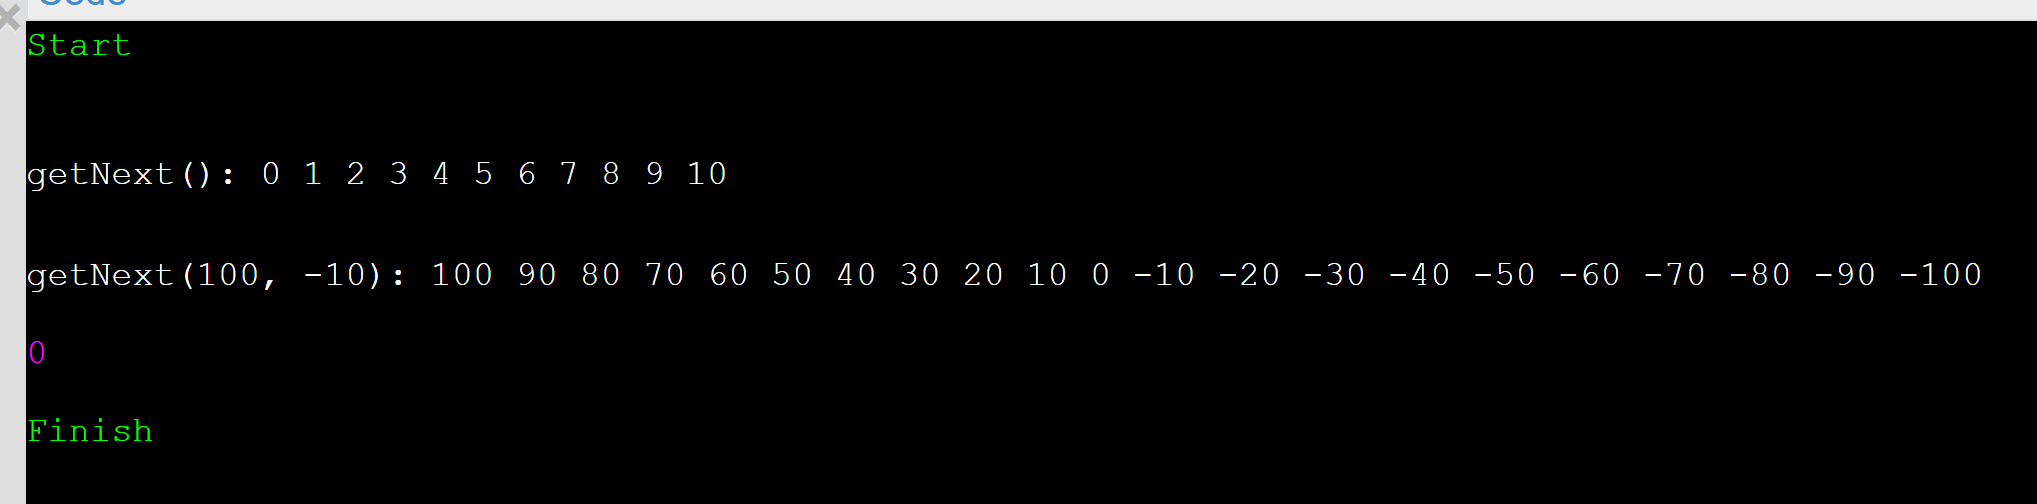
\includegraphics[width=1.0\textwidth]{content/2/chapter3/images/3.png}\\
\end{center}















